\documentclass[tikz,border=4pt]{standalone}

\usepackage{pgfplots}
\pgfplotsset{compat=1.18}
\usetikzlibrary{arrows.meta}

\definecolor{nvidiagreen}{HTML}{76B900}

\begin{document}
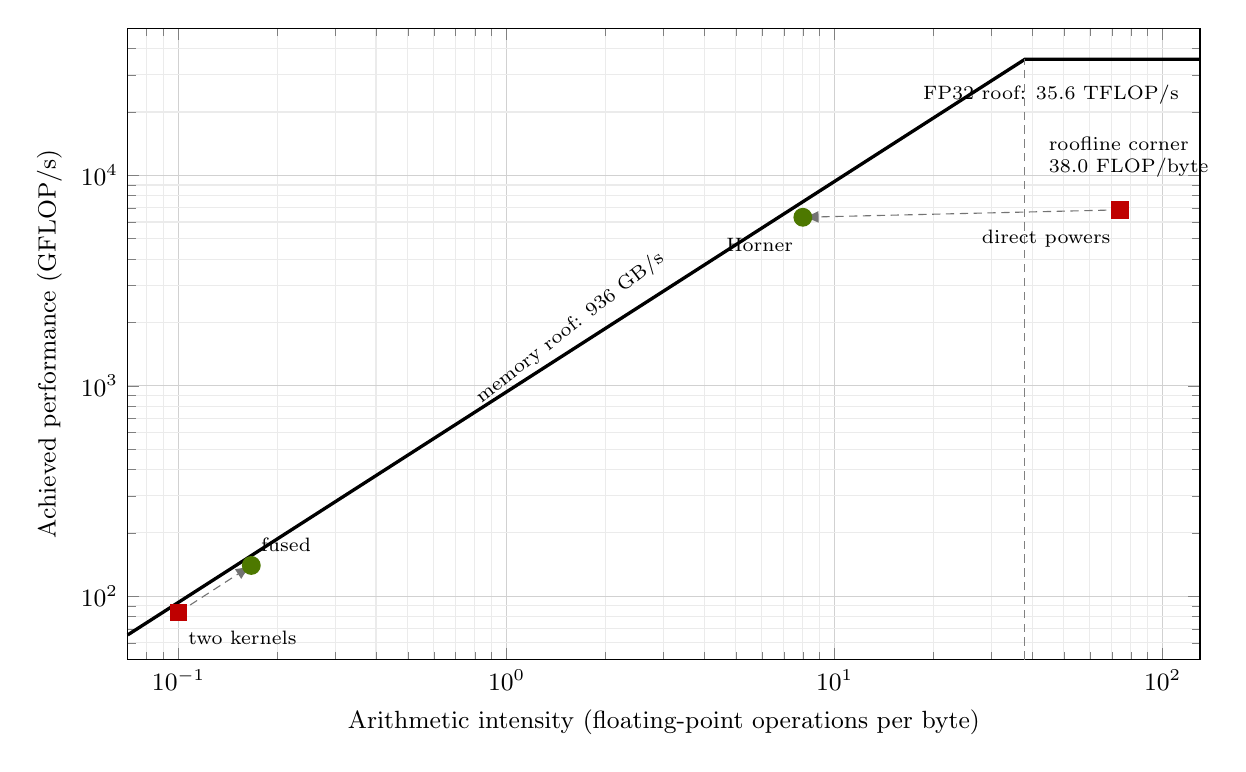
\begin{tikzpicture}
  \begin{loglogaxis}[
    width=15.2cm,
    height=9.6cm,
    xmin=0.07,xmax=130,
    ymin=50,ymax=50000,
    xlabel={Arithmetic intensity (floating-point operations per byte)},
    ylabel={Achieved performance (GFLOP/s)},
    grid=both,
    major grid style={black!18},
    minor grid style={black!8},
    tick label style={font=\small},
    label style={font=\small},
    clip=false]

    % RTX 3090 vendor roofs: 936 GB/s and 35.6 TFLOP/s FP32.
    \addplot[black,very thick]
      coordinates {(0.07,65.52) (0.1,93.6) (1,936) (10,9360)
                   (38.034188,35600) (130,35600)};
    \node[font=\scriptsize,rotate=38,anchor=south]
      at (axis cs:1.7,1591) {memory roof: $936\ \mathrm{GB/s}$};
    \node[font=\scriptsize,anchor=north east]
      at (axis cs:120,30000) {FP32 roof: $35.6\ \mathrm{TFLOP/s}$};

    % The two roofs meet at 35,600 / 936 = 38.034 FLOP/byte.
    \addplot[black!50,densely dashed]
      coordinates {(38.034188,50) (38.034188,35600)};
    \node[font=\scriptsize,anchor=north west,align=left]
      at (axis cs:42,17000) {roofline corner\\$38.0$ FLOP/byte};

    % Dashed arrows connect each baseline to its optimized version.
    \addplot[black!55,densely dashed,-{Latex[length=2mm]}]
      coordinates {(0.1,83.698595) (0.166667,140.073355)};
    \addplot[black!55,densely dashed,-{Latex[length=2mm]}]
      coordinates {(74.25,6856.059418) (8,6319.994726)};

    % Section 3.1: two kernels versus one fused kernel.
    \addplot[only marks,mark=square*,mark size=3pt,
      red!75!black] coordinates {(0.1,83.698595)};
    \node[font=\scriptsize,anchor=north west]
      at (axis cs:0.1,76) {two kernels};
    \addplot[only marks,mark=*,mark size=3.2pt,
      nvidiagreen!65!black] coordinates {(0.166667,140.073355)};
    \node[font=\scriptsize,anchor=south west]
      at (axis cs:0.166667,147) {fused};

    % Section 3.2: direct powers versus Horner's form.
    \addplot[only marks,mark=square*,mark size=3pt,
      red!75!black] coordinates {(74.25,6856.059418)};
    \node[font=\scriptsize,anchor=north east]
      at (axis cs:74.25,6100) {direct powers};
    \addplot[only marks,mark=*,mark size=3.2pt,
      nvidiagreen!65!black] coordinates {(8,6319.994726)};
    \node[font=\scriptsize,anchor=north east]
      at (axis cs:8,5600) {Horner};
  \end{loglogaxis}
\end{tikzpicture}
\end{document}
